\PassOptionsToPackage{unicode=true}{hyperref} % options for packages loaded elsewhere
\PassOptionsToPackage{hyphens}{url}
%
\documentclass[english,man,floatsintext]{apa6}
\usepackage{lmodern}
\usepackage{amssymb,amsmath}
\usepackage{ifxetex,ifluatex}
\usepackage{fixltx2e} % provides \textsubscript
\ifnum 0\ifxetex 1\fi\ifluatex 1\fi=0 % if pdftex
  \usepackage[T1]{fontenc}
  \usepackage[utf8]{inputenc}
  \usepackage{textcomp} % provides euro and other symbols
\else % if luatex or xelatex
  \usepackage{unicode-math}
  \defaultfontfeatures{Ligatures=TeX,Scale=MatchLowercase}
\fi
% use upquote if available, for straight quotes in verbatim environments
\IfFileExists{upquote.sty}{\usepackage{upquote}}{}
% use microtype if available
\IfFileExists{microtype.sty}{%
\usepackage[]{microtype}
\UseMicrotypeSet[protrusion]{basicmath} % disable protrusion for tt fonts
}{}
\IfFileExists{parskip.sty}{%
\usepackage{parskip}
}{% else
\setlength{\parindent}{0pt}
\setlength{\parskip}{6pt plus 2pt minus 1pt}
}
\usepackage{hyperref}
\hypersetup{
            pdftitle={Effects of early language experience on infants' orientation to faces},
            pdfkeywords={keywords},
            pdfborder={0 0 0},
            breaklinks=true}
\urlstyle{same}  % don't use monospace font for urls
\usepackage{graphicx,grffile}
\makeatletter
\def\maxwidth{\ifdim\Gin@nat@width>\linewidth\linewidth\else\Gin@nat@width\fi}
\def\maxheight{\ifdim\Gin@nat@height>\textheight\textheight\else\Gin@nat@height\fi}
\makeatother
% Scale images if necessary, so that they will not overflow the page
% margins by default, and it is still possible to overwrite the defaults
% using explicit options in \includegraphics[width, height, ...]{}
\setkeys{Gin}{width=\maxwidth,height=\maxheight,keepaspectratio}
\setlength{\emergencystretch}{3em}  % prevent overfull lines
\providecommand{\tightlist}{%
  \setlength{\itemsep}{0pt}\setlength{\parskip}{0pt}}
\setcounter{secnumdepth}{0}

% set default figure placement to htbp
\makeatletter
\def\fps@figure{htbp}
\makeatother

% Manuscript styling
\usepackage{upgreek}
\captionsetup{font=singlespacing,justification=justified}

% Table formatting
\usepackage{longtable}
\usepackage{lscape}
% \usepackage[counterclockwise]{rotating}   % Landscape page setup for large tables
\usepackage{multirow}		% Table styling
\usepackage{tabularx}		% Control Column width
\usepackage[flushleft]{threeparttable}	% Allows for three part tables with a specified notes section
\usepackage{threeparttablex}            % Lets threeparttable work with longtable

% Create new environments so endfloat can handle them
% \newenvironment{ltable}
%   {\begin{landscape}\begin{center}\begin{threeparttable}}
%   {\end{threeparttable}\end{center}\end{landscape}}
\newenvironment{lltable}{\begin{landscape}\begin{center}\begin{ThreePartTable}}{\end{ThreePartTable}\end{center}\end{landscape}}

% Enables adjusting longtable caption width to table width
% Solution found at http://golatex.de/longtable-mit-caption-so-breit-wie-die-tabelle-t15767.html
\makeatletter
\newcommand\LastLTentrywidth{1em}
\newlength\longtablewidth
\setlength{\longtablewidth}{1in}
\newcommand{\getlongtablewidth}{\begingroup \ifcsname LT@\roman{LT@tables}\endcsname \global\longtablewidth=0pt \renewcommand{\LT@entry}[2]{\global\advance\longtablewidth by ##2\relax\gdef\LastLTentrywidth{##2}}\@nameuse{LT@\roman{LT@tables}} \fi \endgroup}

% \setlength{\parindent}{0.5in}
% \setlength{\parskip}{0pt plus 0pt minus 0pt}

% \usepackage{etoolbox}
\makeatletter
\patchcmd{\HyOrg@maketitle}
  {\section{\normalfont\normalsize\abstractname}}
  {\section*{\normalfont\normalsize\abstractname}}
  {}{\typeout{Failed to patch abstract.}}
\makeatother
\shorttitle{Language experience and social orientation}
\author{Victoria L Mousley\textsuperscript{1, 2, 3}, Luke Mason\textsuperscript{3}, Tim Smith\textsuperscript{3}, Mairéad MacSweeney\textsuperscript{1, 2}, \& Evelyne Mercure\textsuperscript{1, 2, 3, 4}}
\affiliation{
\vspace{0.5cm}
\textsuperscript{1} UCL Institute of Cognitive Neuroscience\\\textsuperscript{2} UCL Deafness, Cognition and Language Research Centre\\\textsuperscript{3} Birkbeck, University of London\\\textsuperscript{4} Goldsmith's, University of London}
\authornote{Add complete departmental affiliations for each author here. Each new line herein must be indented, like this line.

Enter author note here.


Correspondence concerning this article should be addressed to Victoria L Mousley, Alexandra House, 17 - 19 Queen Square, WC1N 3AZ. E-mail: v.mousley.17@ucl.ac.uk}
\keywords{keywords\newline\indent Word count: X}
\usepackage{lineno}

\linenumbers
\usepackage{csquotes}
\usepackage[titles]{tocloft}
\cftpagenumbersoff{figure}
\renewcommand{\cftfigpresnum}{\itshape\figurename\enspace}
\renewcommand{\cftfigaftersnum}{.\space}
\setlength{\cftfigindent}{0pt}
\setlength{\cftafterloftitleskip}{0pt}
\settowidth{\cftfignumwidth}{Figure 10.\qquad}
\cftpagenumbersoff{table}
\renewcommand{\cfttabpresnum}{\itshape\tablename\enspace}
\renewcommand{\cfttabaftersnum}{.\space}
\setlength{\cfttabindent}{0pt}
\setlength{\cftafterloftitleskip}{0pt}
\settowidth{\cfttabnumwidth}{Table 10.\qquad}
\ifnum 0\ifxetex 1\fi\ifluatex 1\fi=0 % if pdftex
  \usepackage[shorthands=off,main=english]{babel}
\else
  % load polyglossia as late as possible as it *could* call bidi if RTL lang (e.g. Hebrew or Arabic)
  \usepackage{polyglossia}
  \setmainlanguage[]{english}
\fi

\title{Effects of early language experience on infants' orientation to faces}

\date{}

\abstract{
One or two sentences providing a \textbf{basic introduction} to the field, comprehensible to a scientist in any discipline. Two to three sentences of \textbf{more detailed background}, comprehensible to scientists in related disciplines. One sentence clearly stating the \textbf{general problem} being addressed by this particular study. One sentence summarizing the main result (with the words ``\textbf{here we show}'' or their equivalent). Two or three sentences explaining what the \textbf{main result} reveals in direct comparison to what was thought to be the case previously, or how the main result adds to previous knowledge. One or two sentences to put the results into a more \textbf{general context}. Two or three sentences to provide a \textbf{broader perspective}, readily comprehensible to a scientist in any discipline.
}

\begin{document}
\maketitle

\hypertarget{introduction}{%
\section{Introduction}\label{introduction}}

\hypertarget{face-pop-out}{%
\subsection{Face pop-out}\label{face-pop-out}}

Face preference in infancy is important for gathering social information. Infants preferentially orient to face-like stimuli in the first days of life (Farroni et al., 2005; Johnson, 1990). Indeed, the \enquote{face pop-out} effect, infants' preference for faces over objects, persists throughout development (Frank, Vul, \& Johnson, 2009; Gliga, Elsabbagh, Andravizou, \& Johnson, 2009). The original \enquote{face pop-out} task was designed by Gliga et al. (2009), who showed that 6-month-olds make a higher number of and longer duration of fixations to faces over competing stimuli (also see Di Giorgio, Turati, Altoè, \& Simion, 2012). Elsabbagh et al. (2013) replicate this effect, revealing significant face over object preference in 7- to 14-month-olds. Babies were presented with static arrays of a face and four non-social stimuli, including a \enquote{noise} stimulus created from the same face within the array (Elsabbagh et al., 2013). The proportion of trials with infants' first looks to the human face was significantly above chance at both 7-month and 14-month time-points (Elsabbagh et al., 2013).
Using the same face pop-out task, Mercure et al. (2018) show that bilingual infants are faster than monolinguals at orienting to faces. This finding suggests that bilingual infants may be more sensitive than monolingual infants to face versus non-face stimuli. Put another way, bilingual infants' may show a stronger effect of \enquote{attention capture} to faces than do monolingual infants. In the same study, bilingual infants directed more fixations to the face over the non-face stimuli than do monolingual infants (Mercure et al., 2018). Bilingual infants may show stronger \enquote{attention maintenance} (i.e., more fixations) to face over non-face stimuli compared to monolingual infants. It could be that bilinguals' increase in attention capture and maintenance to faces is because bilingual infants rely on facial cues, such as lip patterns, to disambiguate their two native languages. This would lead bilingual infants to orient faster to faces and to scan them more extensively than do monolingual infants, even in the case of still faces, in anticipation of useful mouth movements. This study investigates whether reported bilingual effects for attention capture and maintenance to faces (Mercure et al., 2018) persist past the age of 10 months.
We predict that attention capture (i.e., total face fixation latency) and attention maintence (i.e., total face fixation count) will differ by language group (monolingual vs bilingual). Specifically, we predict that bilingual infants will demonstrate faster fixation latency, calculated as the time from trial onset to first fixation to the face AOI. We also predict that bilingual infants will show significantly higher attention maintenance to the face than monolingual infants. Both predictions are based on Mercure et al. (2018), who show this pattern of effects among younger monolingual and bilingual infants (7 to 10 months of age).
We expect to see a main effect of stimulus category on both fixation latency and fixation count. All babies regardless of language experience should orient more quickly to faces than to objects and return to faces more frequently than to objects. My main hypothesis predicts a Stimulus x Group interaction for both fixation latency and fixation count. For face fixation latency, we expect this significant interaction to be driven by bilingual infants' shorter face AOI latencies than monolinguals. This result would support the notion that bilingual infants orient faster to faces (over objects) compared to monolingual infants. For face fixation count, we predict the significant interaction to be driven by bilingual infants' higher number of visits to the face AOI than monolingual infants. Such a pattern would support the hypothesis that bilingual infants maintain more attention to faces (over objects) compared to monolingual infants.

\hypertarget{faces}{%
\subsection{50 faces}\label{faces}}

**Will add intro re: dynamic face processing literature

\hypertarget{study-1-face-pop-out-methods}{%
\section{Study 1 (Face Pop-Out): Methods}\label{study-1-face-pop-out-methods}}

\hypertarget{participants}{%
\subsection{Participants}\label{participants}}

A total of 18 monolingual (9 girls, mean age = 516.39 days, 16.98 months) and 18 bilingual infants (4 girls, mean age = 507 days, 16.67 months) between 15 and 18 months old contributed data. Monolingual infants were exposed to English (\textgreater{} 95\% exposure) and bilingual infants were exposed to English and one non-English language (\textgreater{} 20\% exposure). The combination of languages varied between infants. Exposure to each language was estimated with an English adaptation (Byers-Heinlein, 2009) of the language exposure questionnaire designed by Bosch and Sebastian-Gallés (1997). Age did not differ between group (\(F(1, 34) = 0.80\), \(\mathit{MSE} = 991.36\), \(p = .377\), \(\hat{\eta}^2_G = .023\)). A further 13 participated in the study but were excluded due to fussiness.

\hypertarget{procedure}{%
\subsection{Procedure}\label{procedure}}

Infants participated in a large study on language experiences which began with five eye-tracking tasks: attention to faces (reported here), as well as tasks for foreign language perception, visual attention, dynamic face processing, and cognitive control. After eye-tracking, participants completed behavioural measures (Mullen Scales of Early Learning and videoed parent-child interaction) and language questionnaires. The protocol required between 1.5 - 2.5 hours per infant including breaks. Only data from the \enquote{attention to faces} task are reported in the present article.
During the \enquote{attention to faces} task, infants sat on their parent's lap in a dimly lit room about 60 cm away from a Tobii TX300 eye-tracker. Infant gaze position was calibrated with colourful animations using a five-point routine. Each infant's gaze and behaviour was monitored throughout the study via webcam. The experimenter occasionally shook a rattle behind the screen to attract the infant's attention.

\hypertarget{stimuli}{%
\subsection{Stimuli}\label{stimuli}}

Eight different slides were presented for 10s each (Elsabbagh et al., 2013; Gliga et al., 2009; Mercure et al., 2018).

\begin{figure}

{\centering \includegraphics[width=3.33in]{/Users/victoriamousley/Desktop/MATLAB/lm_analysis/popout/stimuli/POPOUT1} 

}

\caption{Example of a stimulus silde with five object categories.}\label{fig:taskstim}
\end{figure}

In each slide, five colour images belonging to five object categories: faces, phase-scrambled (\enquote{noise}) faces, birds, cars, and phones (see Figure \ref{fig:taskstim}). Each slide were be presented once and position of stimulus categories were randomised. Images were all of comparable size and presented at an equal distance from the centre of the screen. Differences in colour and luminosity were minimised. Faces all had a direct gaze and happy expression. There were 5 female faces and 3 male faces of different ethnicities. Scrambled faces were created from each face by randomising the phase spectra while maintaining the original outer face contour, with the amplitude and colour spectra remaining constant. For more details about the stimuli, see Elsabbagh et al. (2013). These \enquote{attention to faces} slides were interleaved with blocks from other studies.

\hypertarget{data-analysis}{%
\subsection{Data analysis}\label{data-analysis}}

We used R (Version 3.6.2; R Core Team, 2019) and the R-packages \emph{broom} (Version 0.5.3.9000; Robinson \& Hayes, 2019), \emph{coda} (Version 0.19.3; Plummer, Best, Cowles, \& Vines, 2006), \emph{cowplot} (Version 1.0.0; Wilke, 2019), \emph{dplyr} (Version 0.8.4; Wickham et al., 2019), \emph{e1071} (Version 1.7.3; Meyer, Dimitriadou, Hornik, Weingessel, \& Leisch, 2019), \emph{extrafont} (Version 0.17; Winston Chang, 2014), \emph{forcats} (Version 0.4.0; Wickham, 2019a), \emph{ggplot2} (Version 3.2.1; Wickham, 2016), \emph{ggpubr} (Version 0.2.4; Kassambara, 2019), \emph{gridExtra} (Version 2.3; Auguie, 2017), \emph{kableExtra} (Version 1.1.0; Zhu, 2019), \emph{knitr} (Version 1.28; Xie, 2015), \emph{lme4} (Version 1.1.21; Bates, Mächler, Bolker, \& Walker, 2015), \emph{lmerTest} (Version 3.1.1; Kuznetsova, Brockhoff, \& Christensen, 2017), \emph{magrittr} (Version 1.5; Bache \& Wickham, 2014), \emph{Matrix} (Version 1.2.18; Bates \& Maechler, 2019), \emph{MCMCvis} (Version 0.13.5; Youngflesh, 2018), \emph{naniar} (Version 0.4.2; Tierney, Cook, McBain, \& Fay, 2019), \emph{papaja} (Version 0.1.0.9942; Aust \& Barth, 2018), \emph{plotly} (Version 4.9.1; Sievert, 2018), \emph{praise} (Version 1.0.0; Csardi \& Sorhus, 2015), \emph{purrr} (Version 0.3.3; Henry \& Wickham, 2019), \emph{readr} (Version 1.3.1; Wickham, Hester, \& Francois, 2018), \emph{readxl} (Version 1.3.1; Wickham \& Bryan, 2019), \emph{reshape2} (Version 1.4.3; Wickham, 2007), \emph{showtext} (Version 0.7.1; Qiu \& See file AUTHORS for details., 2020, 2017), \emph{showtextdb} (Version 2.0; Qiu \& See file AUTHORS for details., 2017), \emph{stringr} (Version 1.4.0; Wickham, 2019b), \emph{sysfonts} (Version 0.8; Qiu \& See file AUTHORS for details., 2018), \emph{tibble} (Version 2.1.3; Müller \& Wickham, 2019), \emph{tidyr} (Version 1.0.2; Wickham \& Henry, 2019), and \emph{tidyverse} (Version 1.3.0; Wickham, 2017) for all our analyses. Simulated data, pre-processing scripts, and the pre-registered analysis script can be found on the GitHub repository (Mousley, 2019).

\hypertarget{data-pre-processing}{%
\subsection{Data pre-processing}\label{data-pre-processing}}

We excluded trials where participants looked at the AOIs for less than one cumulative second. Participants were included for analyses if they completed at least five valid trials (Mercure et al., 2018). These criteria are identical to the ones used by Elsabbagh et al. (2013) and Mercure et al. (2018). Five AOIs corresponding to the five stimulus categoires (i.e., faces, scrambled faces, birds, phones, and cars) were defined in MATLAB.
After excluding trials and participants according to the exclusion criteria, fixation latency and fixation count were averaged across all participants' valid trials to normalise for number of completed trials. Fixation latency was defined as the time difference between the trial onset and the first saccade to the face AOI. Fixation count was defined as the number of fixations within each area of interest. Total fixation duration was defined as the total time spent fixating within each area of interest during the trial period of 10s. As we did not have any specific hypotheses regarding group differences in attention to birds, cars, phones, or scrambled faces, these categories were averaged to create a \enquote{non-face} stimulus category. However, any significant face vs non-face effect was followed by planned comparisons for individual contrasts between the face and each object AOI to clarify the stability of the effect across control conditions. For further details, see \enquote{Analysis\_Study2} (Mousley, 2019).

\hypertarget{study-1-face-pop-out-results}{%
\section{Study 1 (Face Pop-Out): Results}\label{study-1-face-pop-out-results}}

\hypertarget{fixation-latency}{%
\subsection{Fixation Latency}\label{fixation-latency}}

The latency between the beginning of each trial and the beginning of the first fixation to face and non-face stimuli was analysed with a 2 (stimulus category: face vs non-face) x 2 (group: monolingual vs bilingual) ANOVA. There was a significant effect of stimulus category (\(F(1, 68) = 49.59\), \(\mathit{MSE} = 0.82\), \(p < .001\)) but not of group (\(F(1, 68) = 2.73\), \(\mathit{MSE} = 0.82\), \(p = .103\)). There was a significant interaction of stimulus category x group (\(F(1, 68) = 10.83\), \(\mathit{MSE} = 0.82\), \(p = .002\)) (see Figure \ref{fig:latencyplot}). Planned latency comparisons of face AOI to each object AOI revealed highly significant effects: car (\(t(54.59) = -6.52\), \(p < .001\)), phone (\(t(57.59) = -8.99\), \(p < .001\)), scrambled face (\(t(67.79) = -6.66\), \(p < .001\)), and bird (\(t(59.12) = -5.36\), \(p < .001\)) (see Figure \ref{fig:lat5plot}).

\begin{figure}
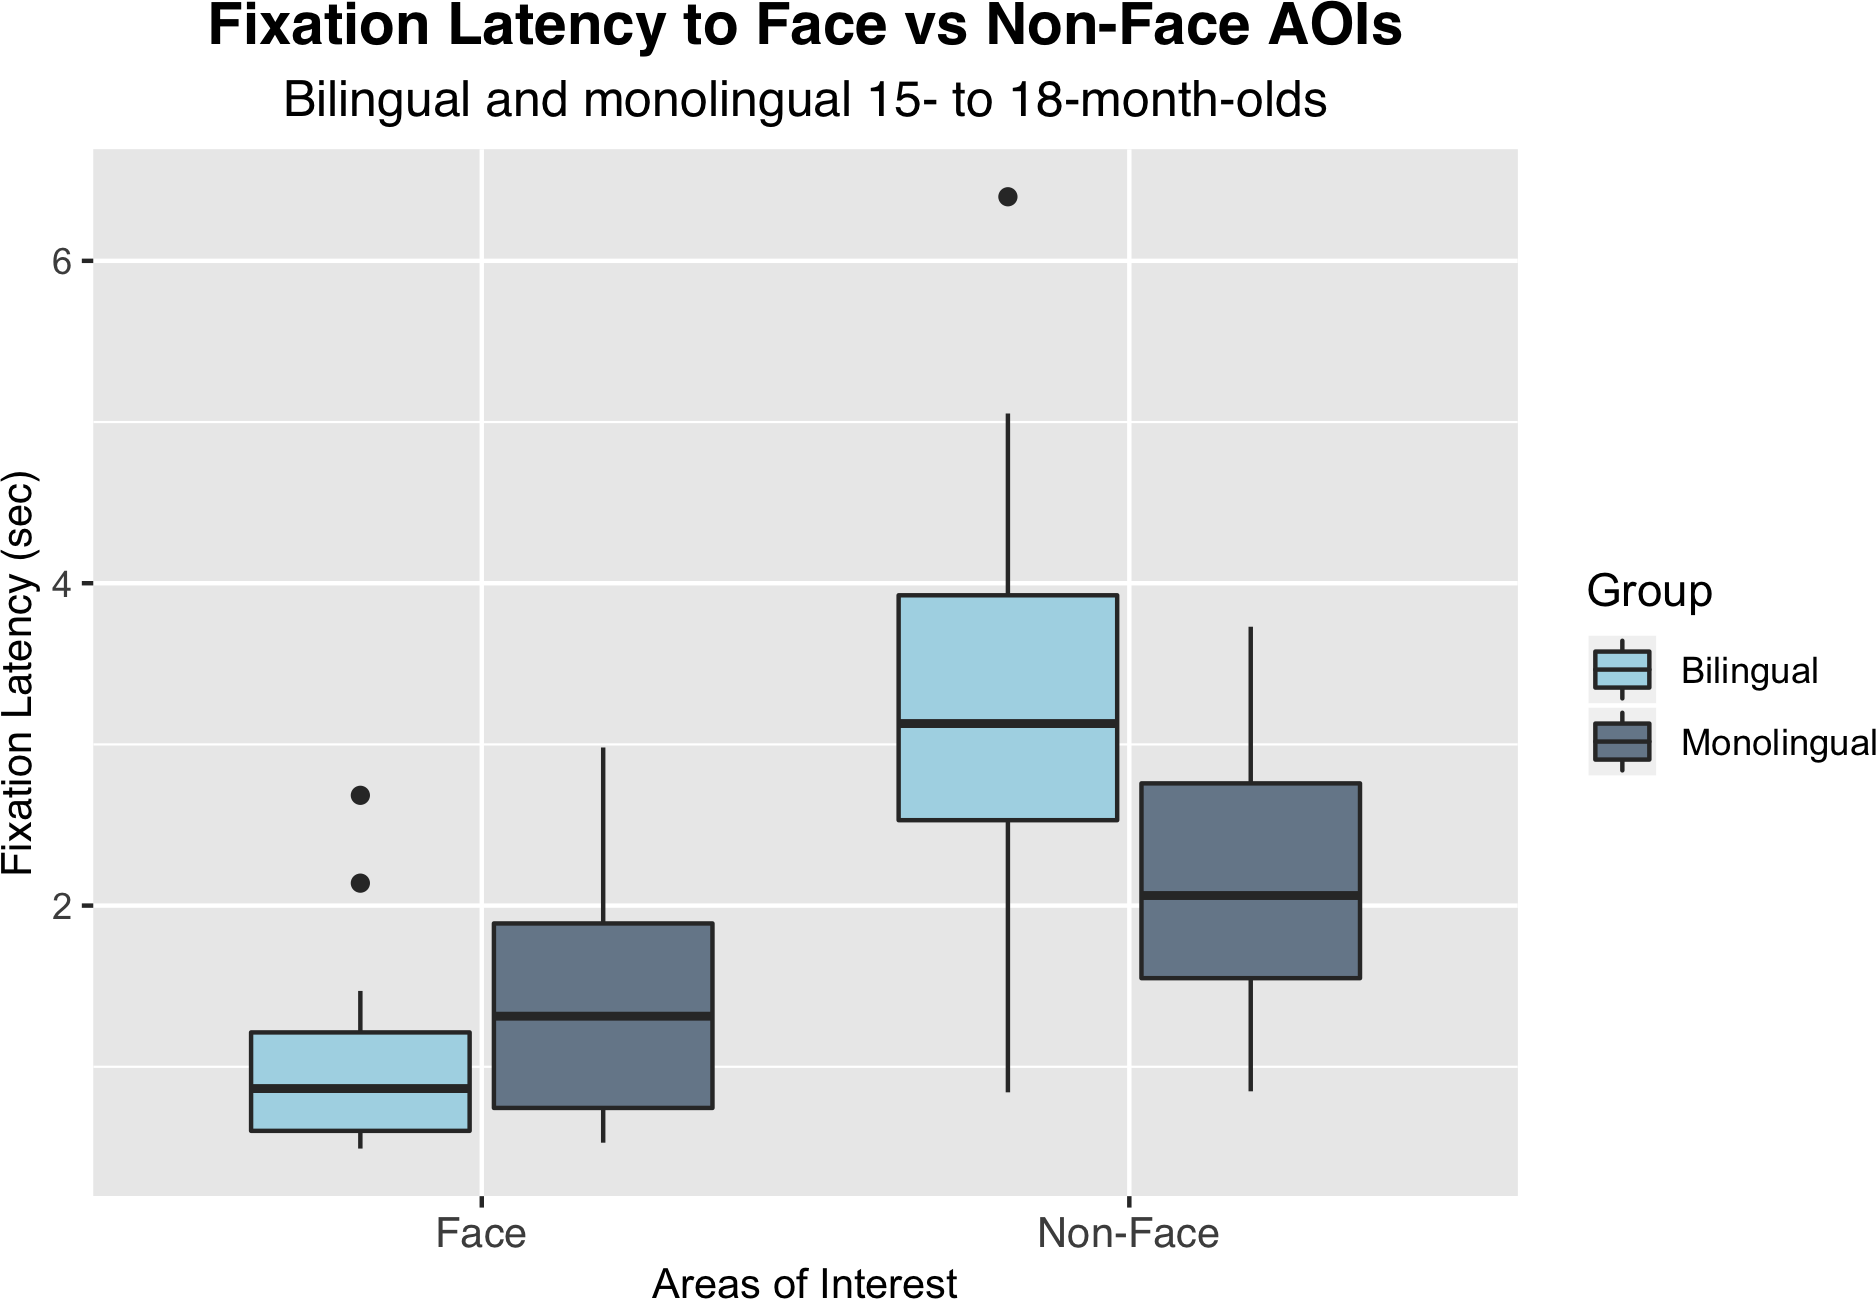
\includegraphics{Effects-of-early-language-experience-on-infants--orientation-to-faces_files/figure-latex/latencyplot-1} \caption{Fixation latency to face vs non-face AOIs by group.}\label{fig:latencyplot}
\end{figure}
\begin{figure}
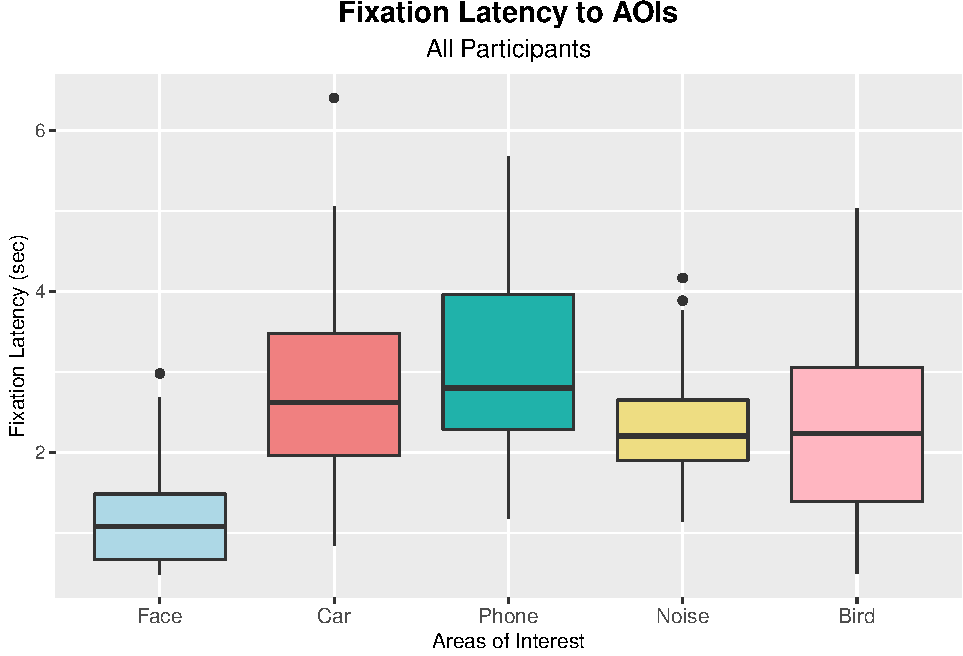
\includegraphics{Effects-of-early-language-experience-on-infants--orientation-to-faces_files/figure-latex/lat5plot-1} \caption{Fixation latency to each AOI across all participants.}\label{fig:lat5plot}
\end{figure}

\hypertarget{fixation-count}{%
\subsection{Fixation Count}\label{fixation-count}}

The number of fixations that infants directed to faces and non-faces was analysed in a 2 (stimulus categories: face vs non-face) x 2 (group: monolingual vs bilingual) ANOVA. A significant effect of stimulus was found {[}\(F(1, 68) = 16.44\), \(\mathit{MSE} = 0.94\), \(p < .001\), \(\hat{\eta}^2_G = .195\){]} but the effect of group was non-significant {[}\(F(1, 68) = 2.73\), \(\mathit{MSE} = 0.94\), \(p = .103\), \(\hat{\eta}^2_G = .039\){]} (see Figure \ref{fig:count2plot}). The interaction of stimulus category x group was non-significant. Planned latency comparisons of face AOI to each object AOI revealed highly significant effects: car (\(t(66.26) = 4.03\), \(p < .001\)), phone (\(t(58.82) = 9.49\), \(p < .001\)), scrambled face (\(t(62.58) = 6.89\), \(p < .001\)), and bird (\(t(69.45) = 4.35\), \(p < .001\)) (see Figure \ref{fig:allcountplot}).

\begin{figure}
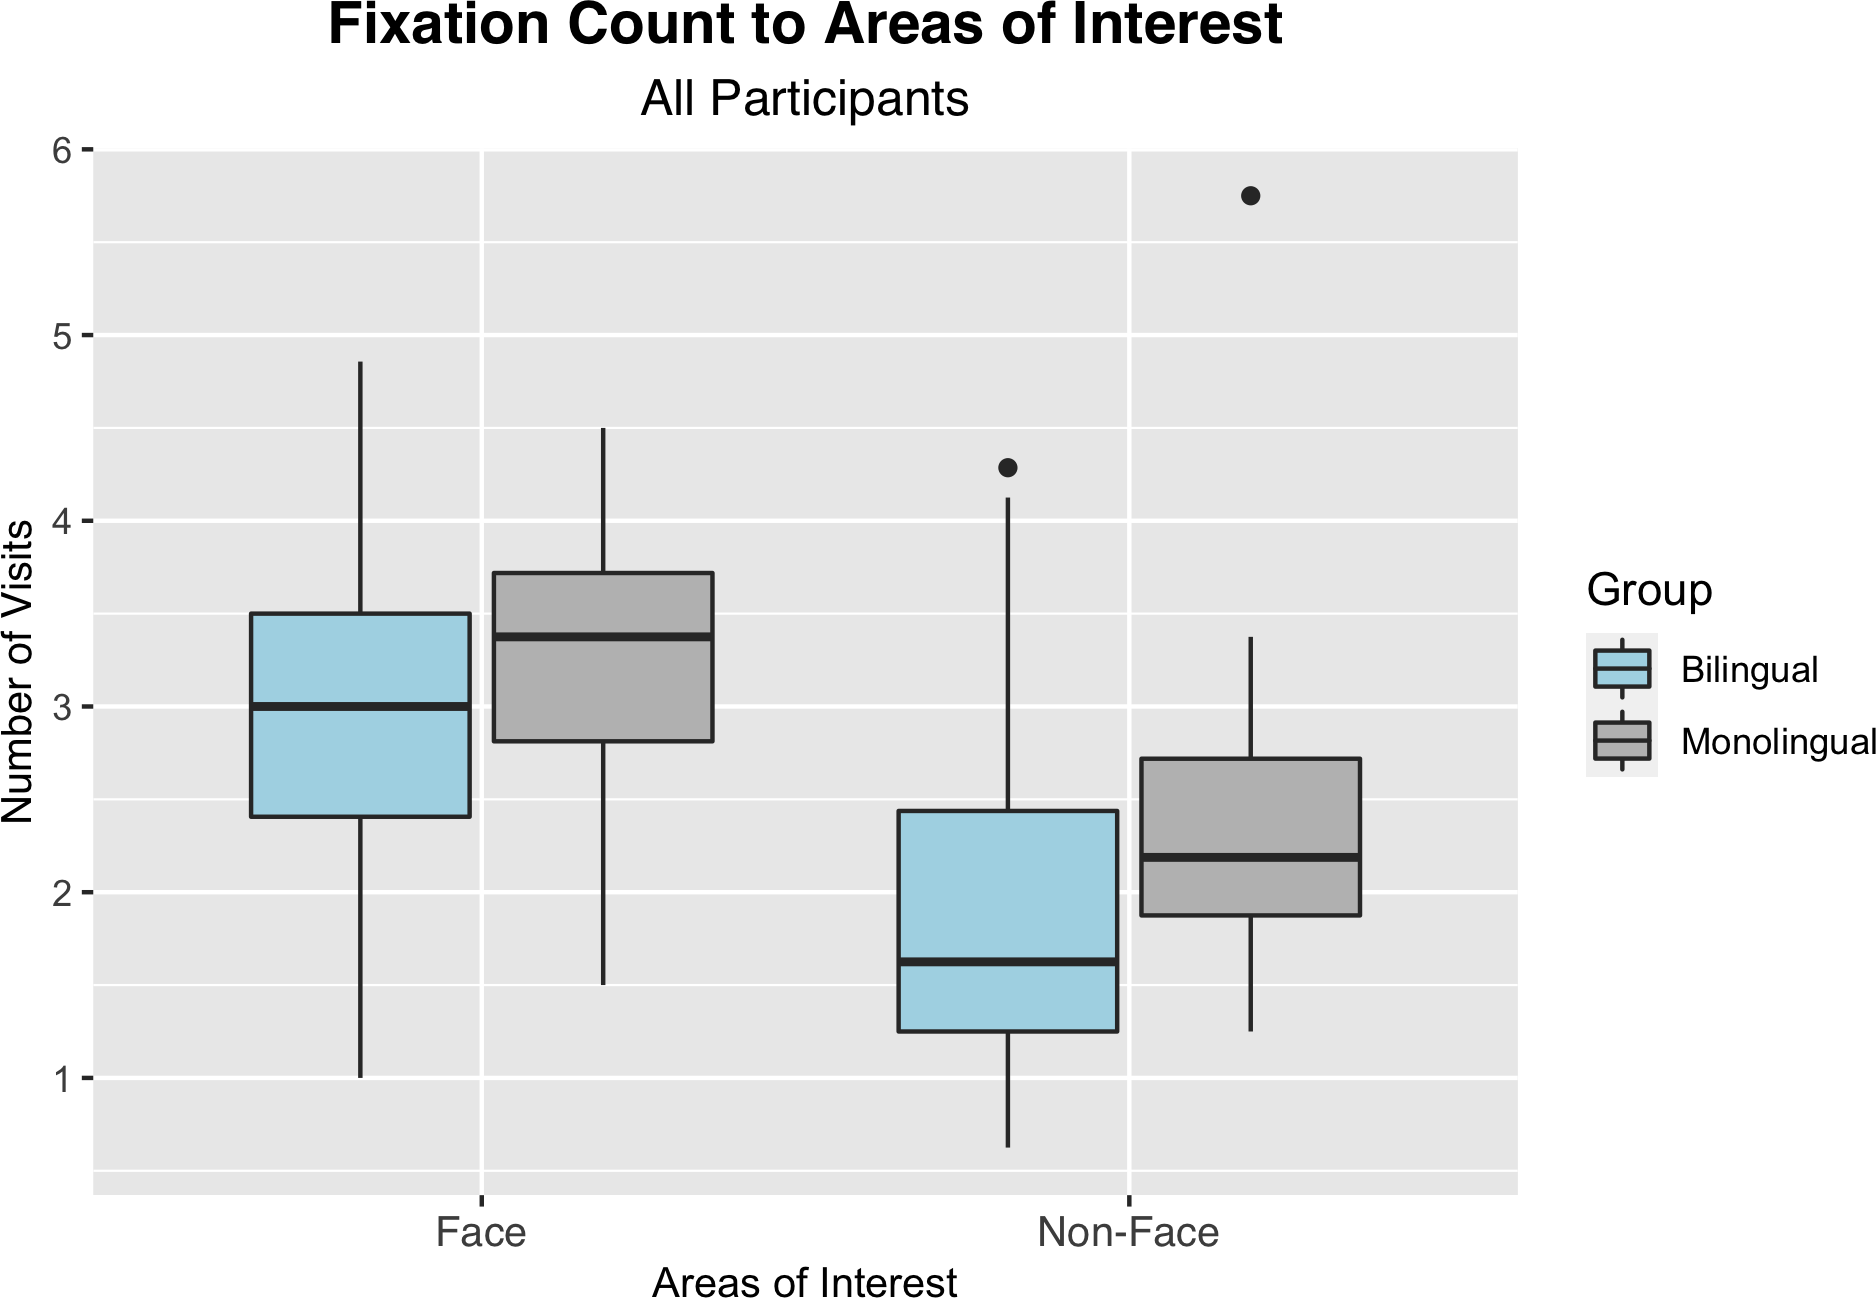
\includegraphics{Effects-of-early-language-experience-on-infants--orientation-to-faces_files/figure-latex/count2plot-1} \caption{Fixation count to face vs non-face stimuli by group.}\label{fig:count2plot}
\end{figure}
\begin{figure}
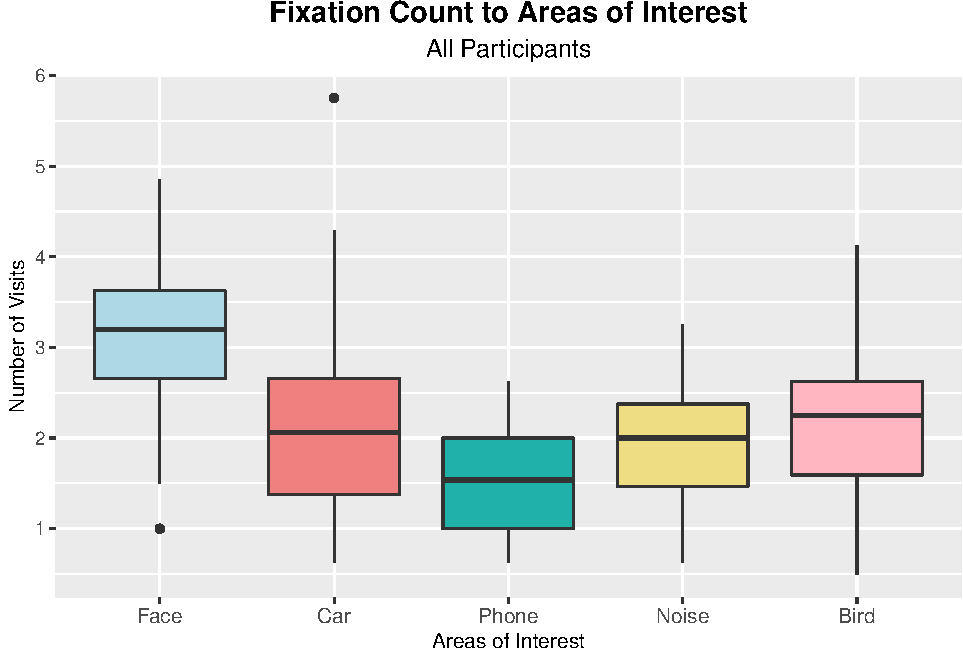
\includegraphics{Effects-of-early-language-experience-on-infants--orientation-to-faces_files/figure-latex/allcountplot-1} \caption{Fixation count to all AOIs across all participants.}\label{fig:allcountplot}
\end{figure}

\hypertarget{fixation-duration}{%
\subsection{Fixation Duration}\label{fixation-duration}}

The total amount of time fixating to faces and non-faces over the whole trial was analysed in a 2 (stimulus category: face vs non-face) x 2 (group: monolingual vs bilingual) ANOVA. A significant effect of stimulus was found (\(F(1, 68) = 3.93\), \(\mathit{MSE} = 1.69\), \(p = .051\), \(\hat{\eta}^2_G = .055\)), but there was no main effect of group or of interaction of stimulus category x group (see Figure \ref{fig:durface}). Infants looked at faces for longer than any of the other object categories. Planned comparisons of face AOI to each object AOI revealed significant effects: phone (\(t(43.35) = 7.60\), \(p < .001\)), car (\(t(68.45) = 2.01\), \(p = .049\)), scrambled face (\(t(49.62) = 6.47\), \(p < .001\)), and bird (\(t(68.82) = 3.27\), \(p = .002\)) (see Figure \ref{fig:alldurplot}).

\begin{figure}
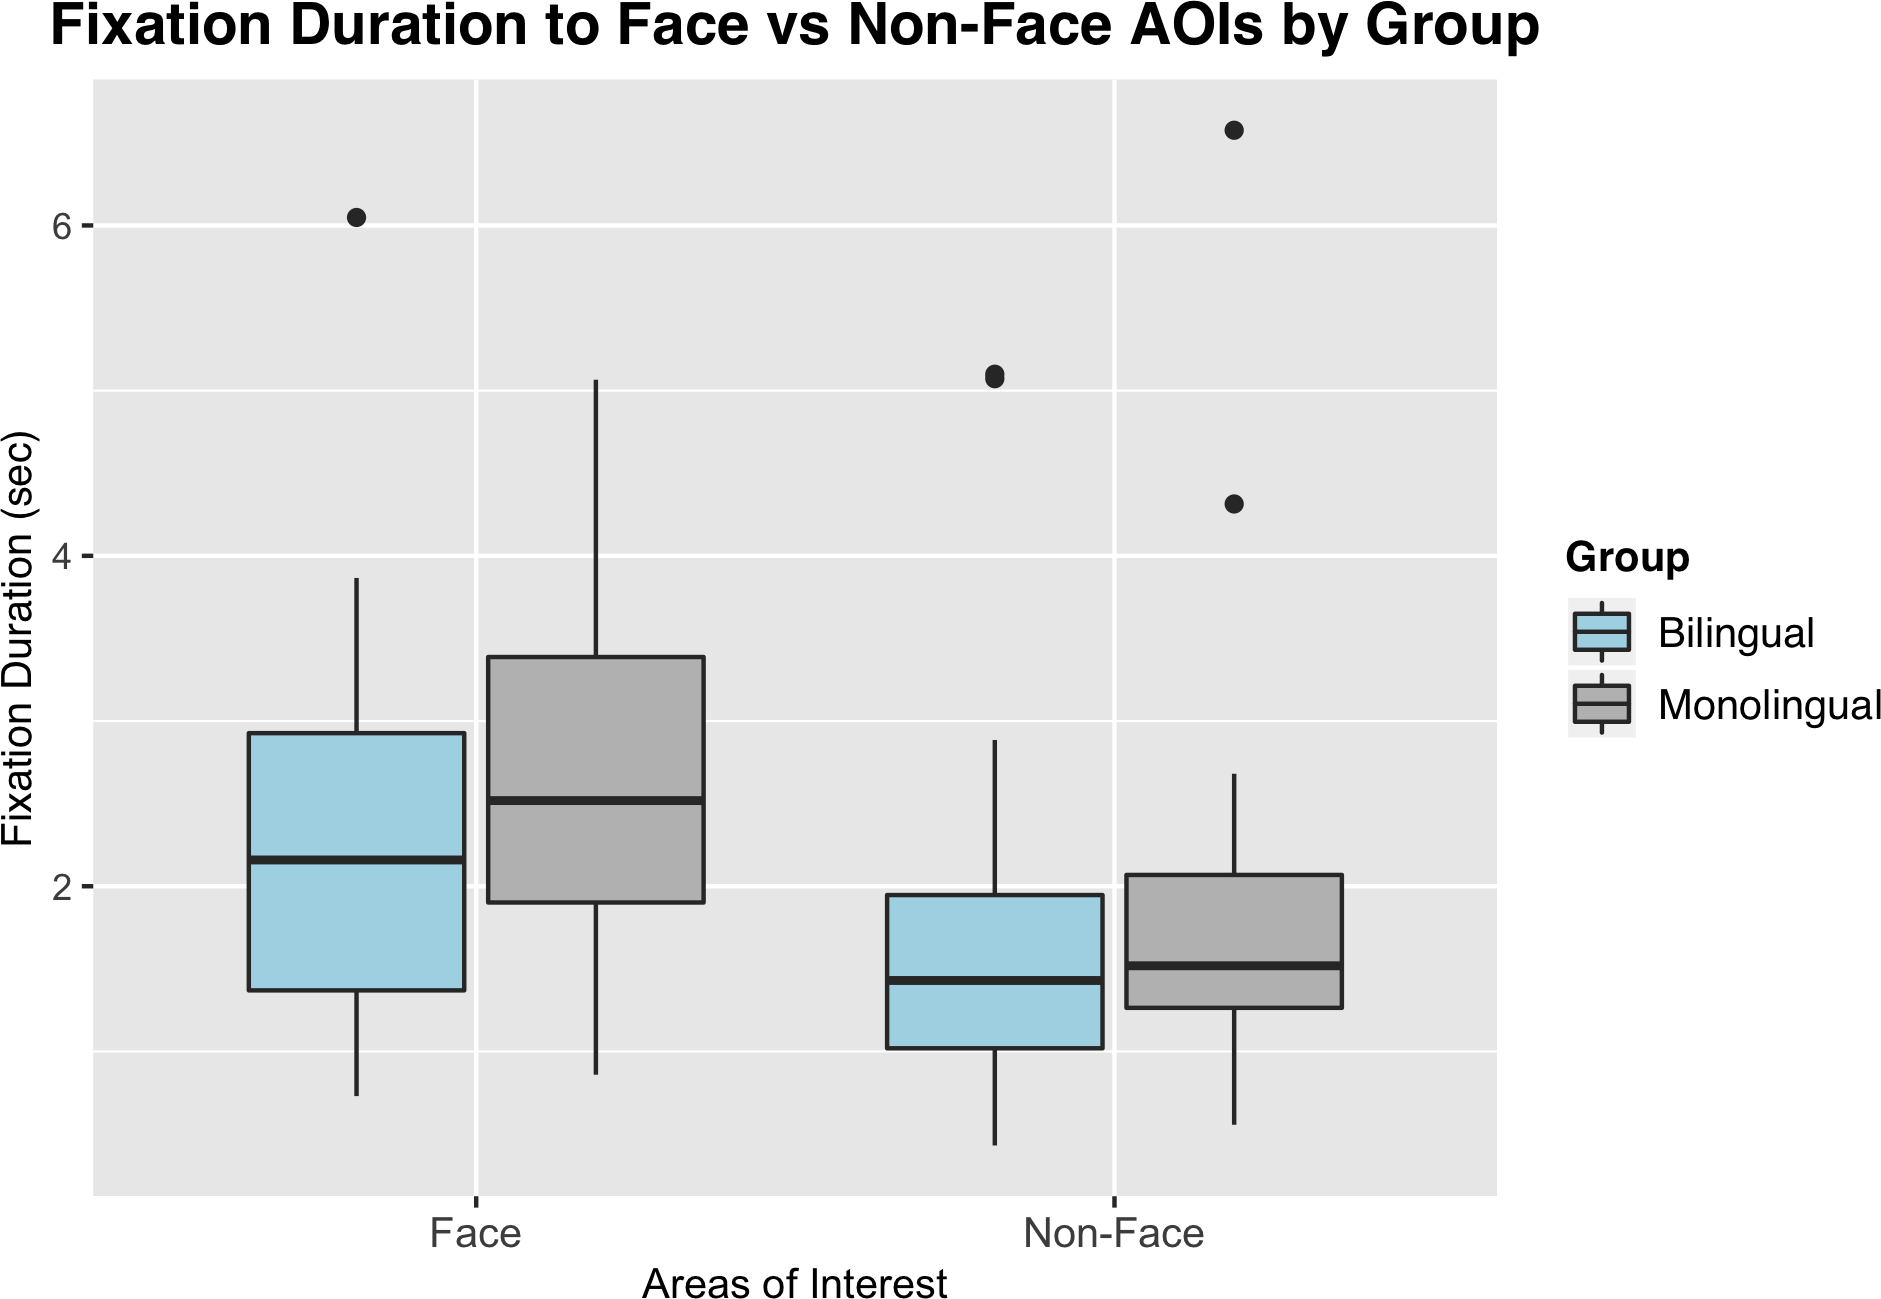
\includegraphics{Effects-of-early-language-experience-on-infants--orientation-to-faces_files/figure-latex/durface-1} \caption{Fixation duration to face vs non-face AOIs by group.}\label{fig:durface}
\end{figure}
\begin{figure}
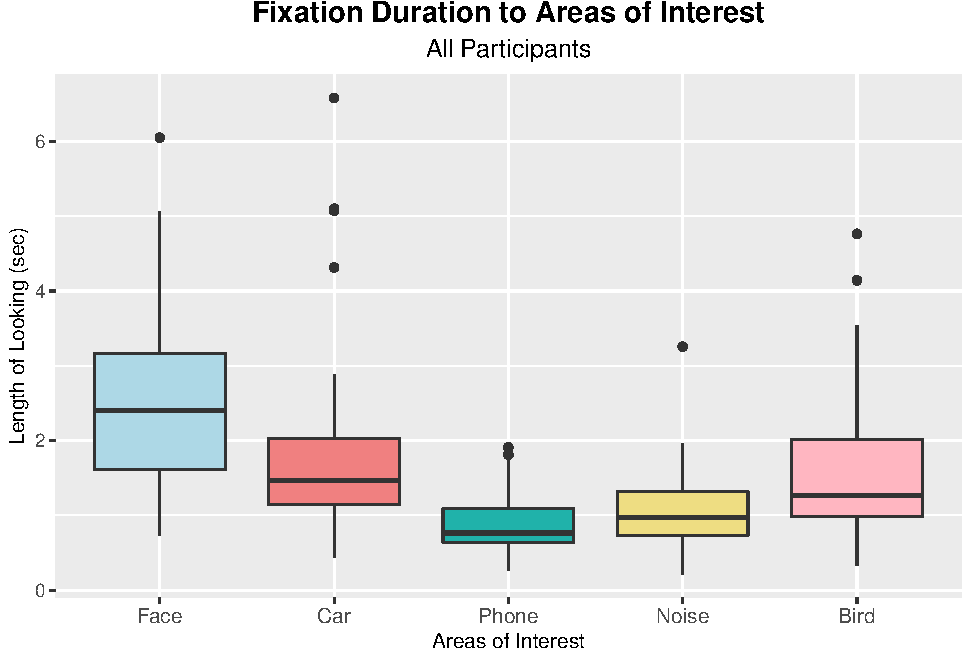
\includegraphics{Effects-of-early-language-experience-on-infants--orientation-to-faces_files/figure-latex/alldurplot-1} \caption{Fixation duration to AOIs across all participants.}\label{fig:alldurplot}
\end{figure}

\hypertarget{face-orientation-index}{%
\subsection{Face Orientation Index}\label{face-orientation-index}}

A index of \enquote{face orientation} (FO) was calculated with the following formula: non-face latency - face latency / non-face latency + face latency. A generalised linear model revealed non-significant effects of age {[}\(t(32) = -1.09\), \(p = .285\){]}, group {[}\(t(32) = -0.84\), \(p = .409\){]}, and interaction {[}\(t(32) = 0.69\), \(p = .496\){]}.

\begin{figure}
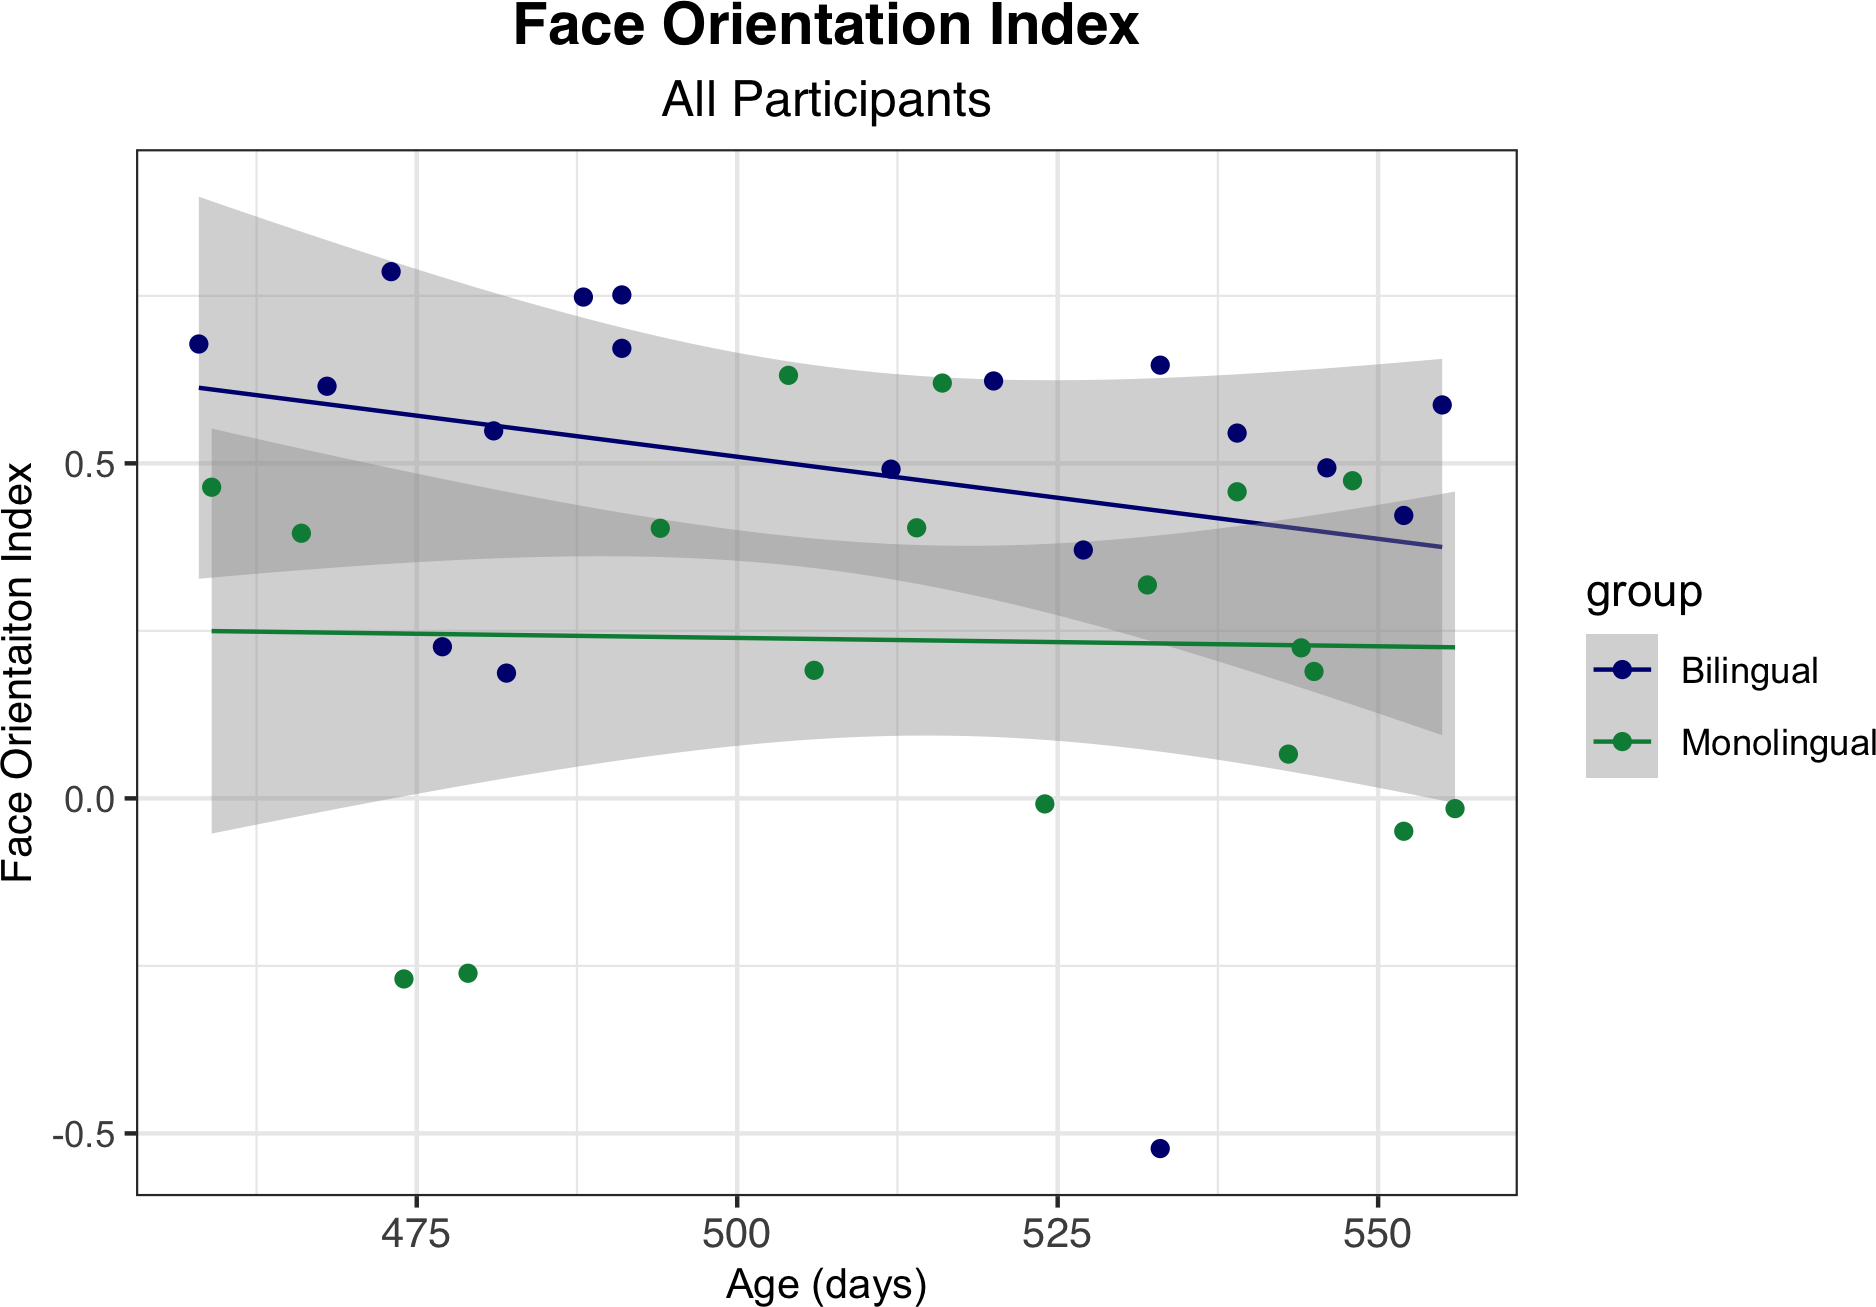
\includegraphics{Effects-of-early-language-experience-on-infants--orientation-to-faces_files/figure-latex/FOM-1} \caption{Face orientation index by group.}\label{fig:FOM}
\end{figure}

** Note to Evelyne: I can include FOI analyses on your face pop-out if you want, but I would need the data.

\hypertarget{study-2-50-faces-methods}{%
\section{Study 2 (50 Faces): Methods}\label{study-2-50-faces-methods}}

\hypertarget{participants-1}{%
\subsection{Participants}\label{participants-1}}

\hypertarget{sample-1-evelynes-sample}{%
\subsubsection{Sample 1 (Evelyne's Sample)}\label{sample-1-evelynes-sample}}

A total of 24 monolingual (14 girls, mean age = 265.33 days, 8.72 months) and 24 bilingual infants (10 girls, mean age = 256.12 days, 8.42 months) between 7 and 10 months old contributed data. Monolingual infants were exposed to English (\textgreater{} 95\% exposure) and bilingual infants were exposed to English and one non-English language (\textgreater{} 20\% exposure). The combination of languages varied between infants. Exposure to each language was estimated with an English adaptation (Byers-Heinlein, 2009) of the language exposure questionnaire designed by Bosch and Sebastian-Gallés (1997). Age did not differ between group (\(F(1, 46) = 1.95\), \(\mathit{MSE} = 523.04\), \(p = .170\), \(\hat{\eta}^2_G = .041\)). A further 4 participated in the study but were excluded due to fussiness.

\hypertarget{sample-2-victorias-sample}{%
\subsubsection{Sample 2 (Victoria's Sample)}\label{sample-2-victorias-sample}}

A total of 27 monolingual (11 girls, mean age = 513.89 days, 16.90 months) and 26 bilingual infants (11 girls, mean age = 506.58 days, 16.65 months) between 15 and 18 months old contributed data. Monolingual infants were exposed to English (\textgreater{} 95\% exposure) and bilingual infants were exposed to English and one non-English language (\textgreater{} 20\% exposure). The combination of languages varied between infants. Exposure to each language was estimated with an English adaptation (Byers-Heinlein, 2009) of the language exposure questionnaire designed by Bosch and Sebastian-Gallés (1997). Age did not differ between group (\(F(1, 51) = 0.72\), \(\mathit{MSE} = 977.94\), \(p = .399\), \(\hat{\eta}^2_G = .014\)). A further 4 participated in the study but were excluded due to fussiness.
Infants' parents were contacted from the Birkbeck Babylab database of primarily London-based volunteers recruited from advertisements and mum-and-baby groups, parenting websites, and publications. Parents reported no hearing problems or vision problems, and no serious mental or physical conditions. Travel expenses were reimbursed, and a young scientist t-shirt and certificate of participation were offered to families.
This study was carried out in accordance with the UCL and Birkbeck Research Ethics Committees and conforms with the General Data Protection Regulation (2018). All parents gave written informed consent prior to participation.

\hypertarget{procedure-1}{%
\subsection{Procedure}\label{procedure-1}}

*Will write this once I figure out the best way to organise sections\ldots{}

\hypertarget{stimuli-1}{%
\subsection{Stimuli}\label{stimuli-1}}

*Will write this.

\hypertarget{study-2-50-faces-results}{%
\section{Study 2 (50 Faces): Results}\label{study-2-50-faces-results}}

\hypertarget{proportion-of-looking-to-the-mouth}{%
\subsection{Proportion of looking to the mouth}\label{proportion-of-looking-to-the-mouth}}

\hypertarget{sample-1-evelynes-data-7---10-months}{%
\subsubsection{Sample 1 (Evelyne's Data: 7 - 10 months)}\label{sample-1-evelynes-data-7---10-months}}

A t-test revealed no significant difference between monolingual and bilingual infants' proportion of looking to the mouth. A generalised linear model revealed non-significant effects of age {[}\(t(44) = 0.57\), \(p = .571\){]}, group {[}\(t(44) = 0.32\), \(p = .751\){]}, and interaction {[}\(t(44) = -0.36\), \(p = .724\){]} (see Figure @ref(fig:mouthpropplot\_em).
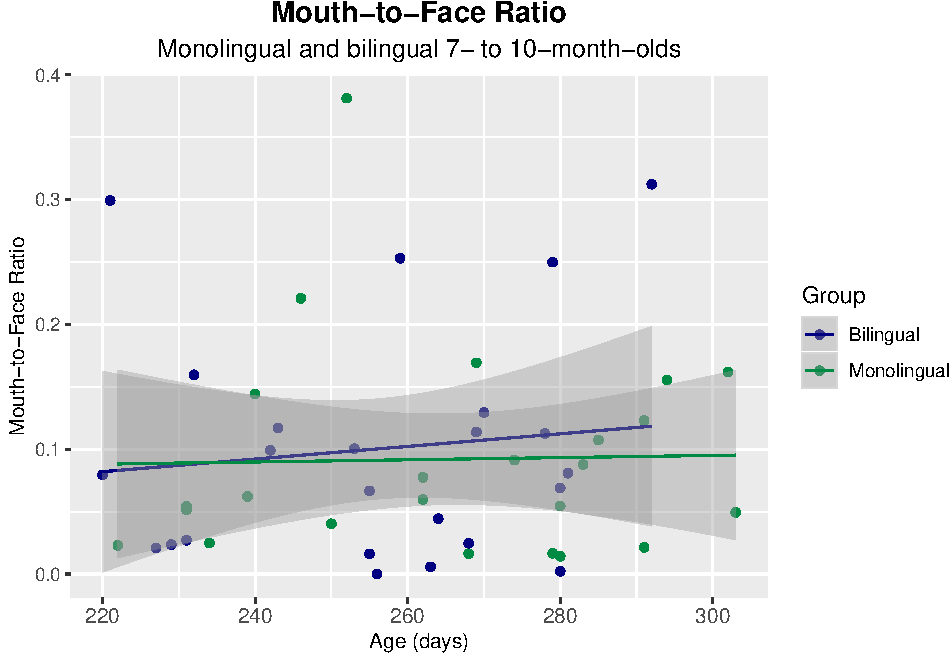
\includegraphics{Effects-of-early-language-experience-on-infants--orientation-to-faces_files/figure-latex/mouthpropplot_em-1.pdf}

\hypertarget{sample-2-victorias-data-15---18-months}{%
\subsubsection{Sample 2 (Victoria's Data: 15 - 18 months)}\label{sample-2-victorias-data-15---18-months}}

A t-test revealed no significant difference between monolingual and bilingual infants' proportion of looking time to the mouth. A generalised linear model revealed non-significant effects of age {[}\(t(49) = 1.54\), \(p = .130\){]}, age {[}\(t(49) = 1.38\), \(p = .172\){]}, and interaction {[}\(t(49) = -1.32\), \(p = .192\){]} (see Figure @ref(fig:vm\_mouthpropplot)).
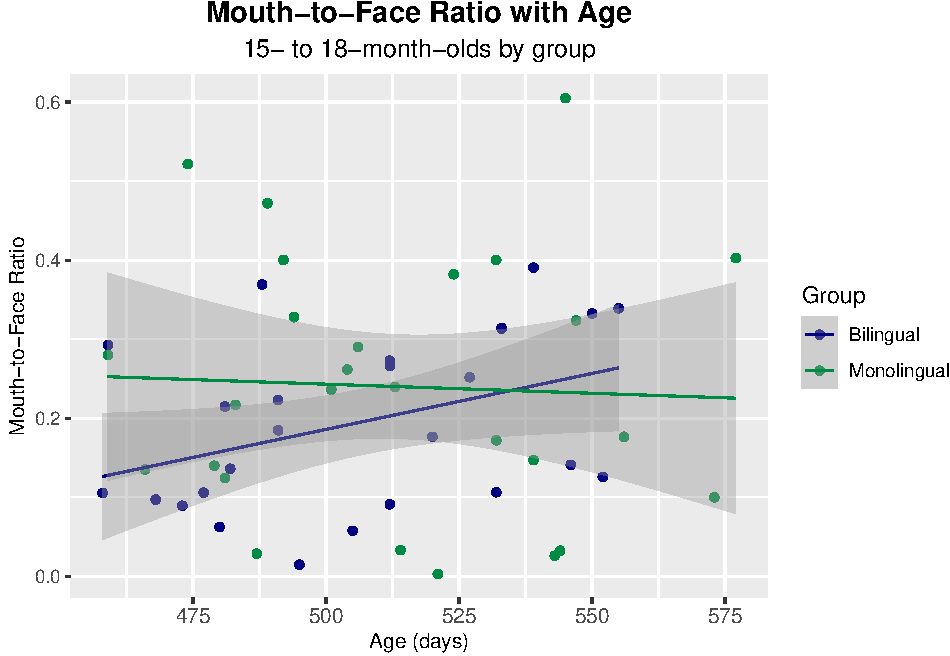
\includegraphics{Effects-of-early-language-experience-on-infants--orientation-to-faces_files/figure-latex/vm_mouthpropplot-1.pdf}

\hypertarget{combined-sample-1-sample-2}{%
\subsubsection{Combined Sample 1 \& Sample 2}\label{combined-sample-1-sample-2}}

****Need to do this.

\hypertarget{total-looking-time-to-mouth}{%
\subsection{Total looking time to mouth}\label{total-looking-time-to-mouth}}

\hypertarget{sample-1-evelynes-data-7---10-months-1}{%
\subsubsection{Sample 1 (Evelyne's Data: 7 - 10 months)}\label{sample-1-evelynes-data-7---10-months-1}}

A t-test revealed no significant difference between monolingual and bilingual infants' total looking time to the mouth. A generalised linear model revealed non-significant effects of age {[}\(t(44) = 0.88\), \(p = .384\){]}, group {[}\(t(44) = 0.54\), \(p = .590\){]}, and interaction {[}\(t(44) = -0.58\), \(p = .568\){]} (see Figure @ref(fig:em\_mouthLTplot)).
\textbackslash{}begin\{figure\}
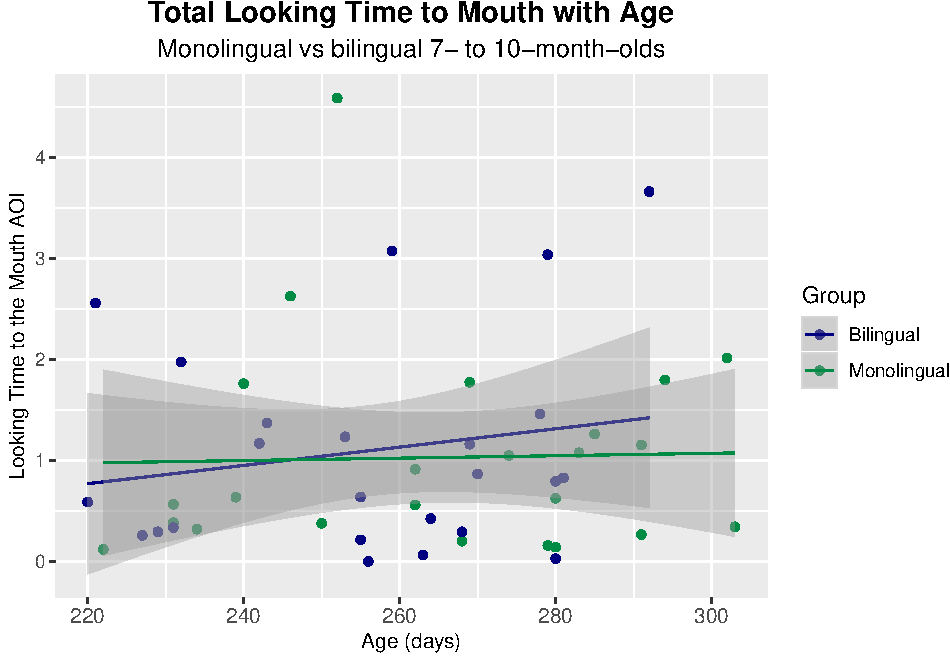
\includegraphics{Effects-of-early-language-experience-on-infants--orientation-to-faces_files/figure-latex/em_mouthLTplot-1}

\caption{Total looking to mouth AOI with age.}

(\#fig:em\_mouthLTplot)
\textbackslash{}end\{figure\}

\hypertarget{sample-2-victorias-data-15---18-months-1}{%
\subsubsection{Sample 2 (Victoria's Data: 15 - 18 months)}\label{sample-2-victorias-data-15---18-months-1}}

A t-test revealed no significant difference between monolingual and bilingual infants' total looking time to the mouth. A generalised linear model showed non-significant effects of age {[}\(t(49) = 1.41\), \(p = .165\){]}, group {[}\(t(49) = 1.45\), \(p = .155\){]}, and interaction {[}\(t(49) = -1.37\), \(p = .176\){]} (see Figure @ref(fig:vm\_mouthLT)).
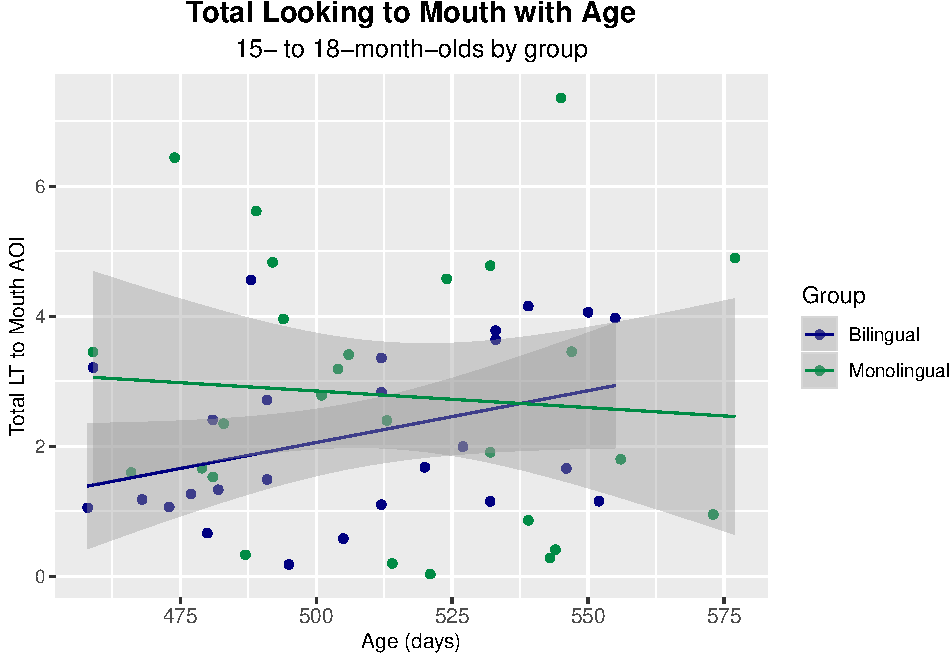
\includegraphics{Effects-of-early-language-experience-on-infants--orientation-to-faces_files/figure-latex/vm_mouthLT-1.pdf}

\hypertarget{combined-sample-1-sample-2-1}{%
\subsubsection{Combined Sample 1 \& Sample 2}\label{combined-sample-1-sample-2-1}}

****Need to do this.

\hypertarget{total-looking-time-to-face}{%
\subsection{Total looking time to face}\label{total-looking-time-to-face}}

\hypertarget{sample-1-evelynes-data-7---10-months-2}{%
\subsubsection{Sample 1 (Evelyne's Data: 7 - 10 months)}\label{sample-1-evelynes-data-7---10-months-2}}

A t-test revealed no significant difference between monolingual and bilingual infants' total looking time to the face. A generalised linear model revealed non-significant effects of age {[}\(t(44) = 0.62\), \(p = .538\){]}, group {[}\(t(44) = 0.03\), \(p = .980\){]}, and interaction {[}\(t(44) = -0.09\), \(p = .930\){]} (see Figure @ref(fig:em\_faceLTAvplot)).
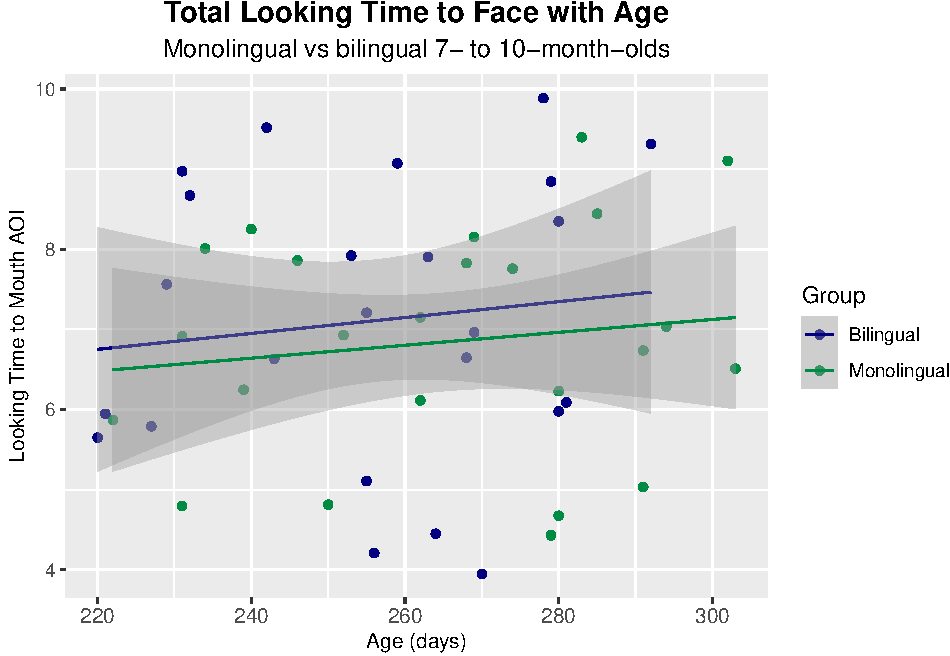
\includegraphics{Effects-of-early-language-experience-on-infants--orientation-to-faces_files/figure-latex/em_faceLTAvplot-1.pdf}

\hypertarget{sample-2-victorias-data-15---18-months-2}{%
\subsubsection{Sample 2 (Victoria's Data: 15 - 18 months)}\label{sample-2-victorias-data-15---18-months-2}}

A t-test revealed no significant difference between monolingual and bilingual infants' total looking time to the face. A generalised linear model revealed non-significant effects of age {[}\(t(49) = 0.42\), \(p = .677\){]}, group {[}\(t(49) = 1.09\), \(p = .281\){]}, and interaction {[}\(t(49) = -1.08\), \(p = .287\){]} (see Figure @ref(fig:vm\_faceLTAvListplot)).
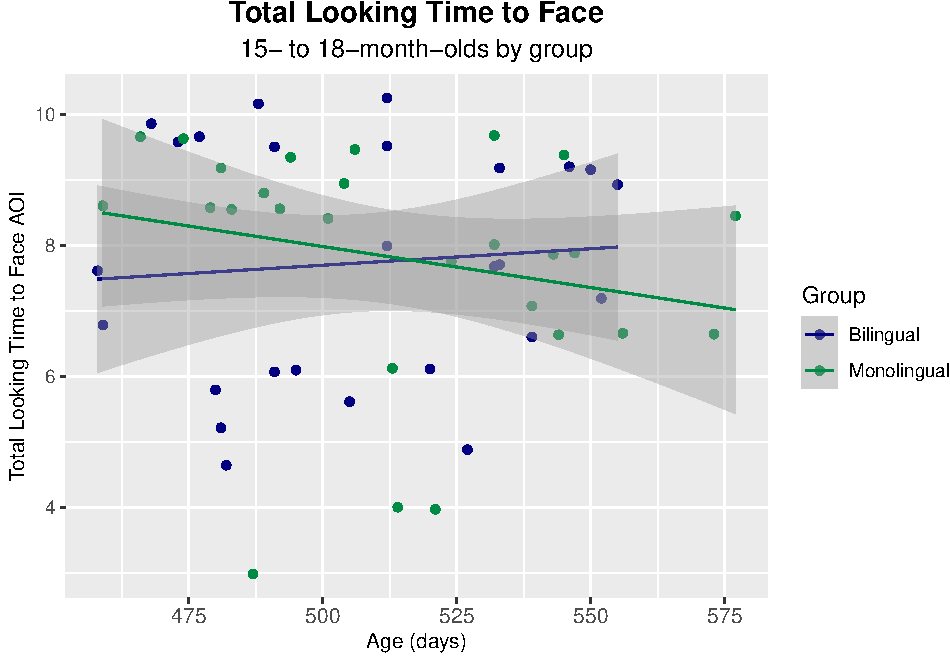
\includegraphics{Effects-of-early-language-experience-on-infants--orientation-to-faces_files/figure-latex/vm_faceLTAvListplot-1.pdf}

\hypertarget{combined-sample-1-sample-2-2}{%
\subsubsection{Combined Sample 1 \& Sample 2}\label{combined-sample-1-sample-2-2}}

****Need to do this.

\hypertarget{eyes-to-face-ratio}{%
\subsection{Eyes-to-face ratio}\label{eyes-to-face-ratio}}

\hypertarget{sample-1-evelynes-data-7---10-months-3}{%
\subsubsection{Sample 1 (Evelyne's Data: 7 - 10 months)}\label{sample-1-evelynes-data-7---10-months-3}}

A t-test revealed no significant difference between monolingual and bilingual infants' eyes-to-face ratio. A generalised linear model revealed non-significant effects of age {[}\(t(44) = 0.68\), \(p = .500\){]}, group {[}\(t(44) = 0.07\), \(p = .943\){]}, and interaction {[}\(t(44) = -0.12\), \(p = .903\){]} (see Figure @ref(fig:em\_e2fplot)).
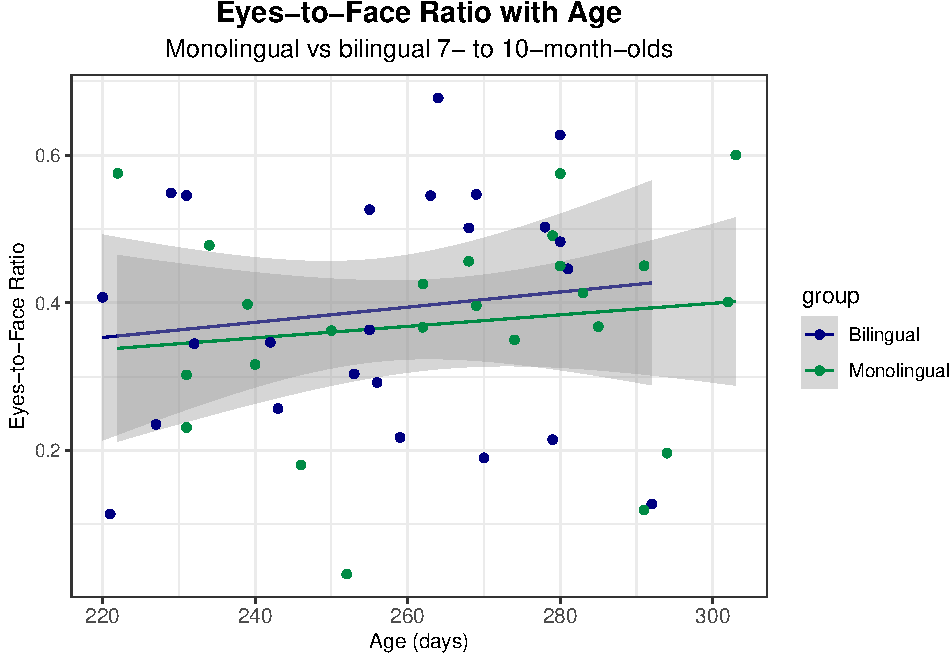
\includegraphics{Effects-of-early-language-experience-on-infants--orientation-to-faces_files/figure-latex/em_e2fplot-1.pdf}

\hypertarget{sample-2-victorias-data-15---18-months-3}{%
\subsubsection{Sample 2 (Victoria's Data: 15 - 18 months)}\label{sample-2-victorias-data-15---18-months-3}}

A t-test revealed no significant difference between monolingual and bilingual infants' eyes-to-face ratio. A generalised linear model revealed a significant effect of age {[}\(t(49) = -1.97\), \(p = .055\){]}, and a non-significant main effect of group {[}\(t(49) = -1.56\), \(p = .126\){]} and interaction {[}\(t(49) = 1.50\), \(p = .139\){]} (see Figure @red(fig:vm\_e2fplot)).
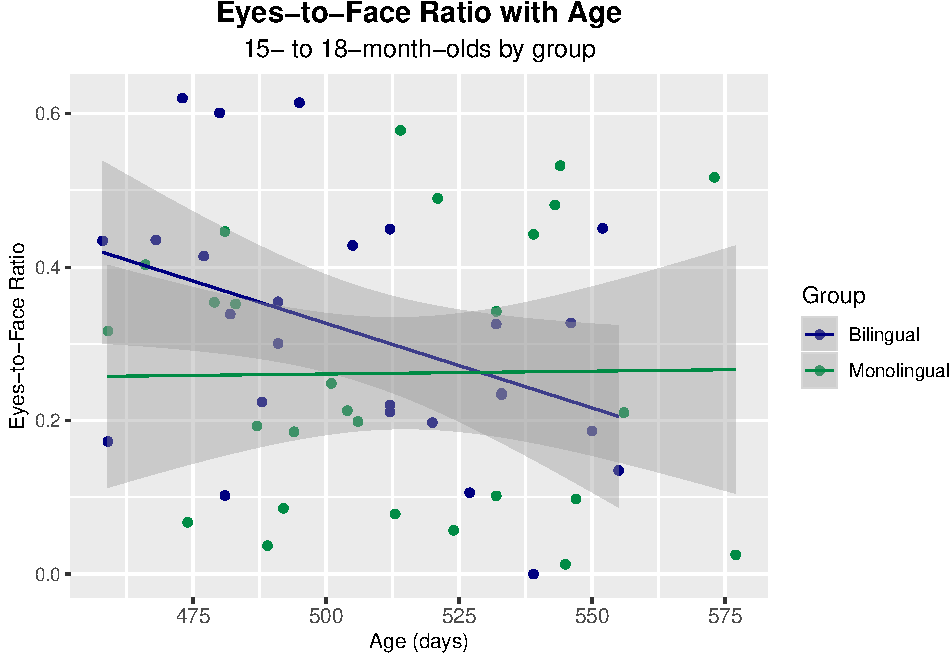
\includegraphics{Effects-of-early-language-experience-on-infants--orientation-to-faces_files/figure-latex/vm_e2fplot-1.pdf}

\hypertarget{mouth-to-face-ratio}{%
\subsection{Mouth-to-face ratio}\label{mouth-to-face-ratio}}

\hypertarget{sample-1-evelynes-data-7---10-months-4}{%
\subsubsection{Sample 1 (Evelyne's Data: 7 - 10 months)}\label{sample-1-evelynes-data-7---10-months-4}}

A t-test revealed no significant difference between monolingual and bilingual infants' mouth-to-face ratio. A generalised linear model revealed non-significant effects of age {[}{]}, group {[}{]}, and interaction {[}{]} (see Figure @ref(fig:em\_m2fplot)).
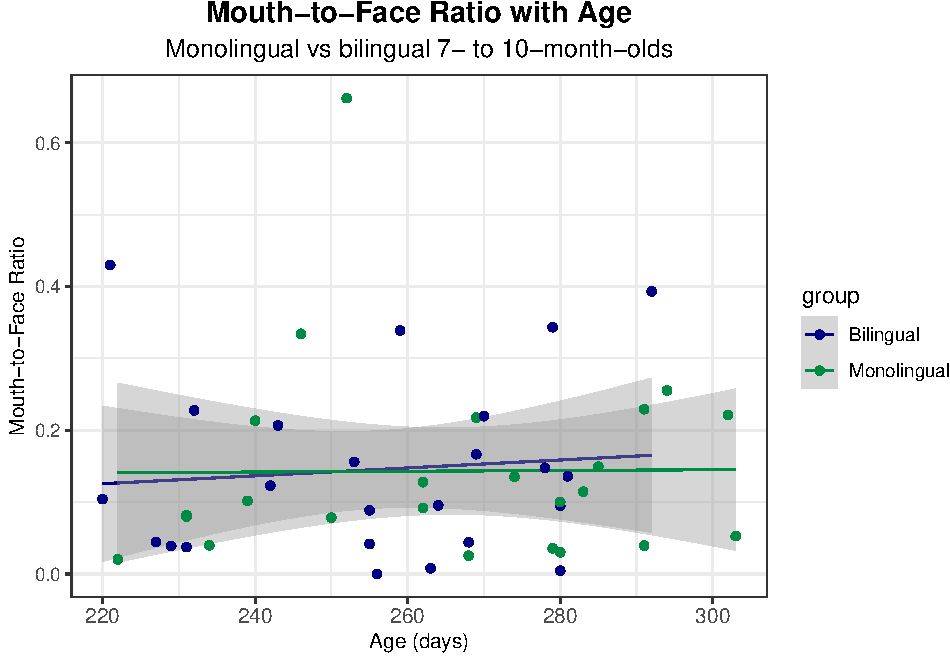
\includegraphics{Effects-of-early-language-experience-on-infants--orientation-to-faces_files/figure-latex/em_m2fplot-1.pdf}

\hypertarget{sample-2-victorias-data-15---18-months-4}{%
\subsection{Sample 2 (Victoria's Data: 15 - 18 months)}\label{sample-2-victorias-data-15---18-months-4}}

A t-test revealed no significant difference between monolingual and bilingual infants' mouth-to-face ratio. A generalised linear model revealed non-significant effects of age {[}\(t(49) = 1.35\), \(p = .184\){]}, group {[}\(t(49) = 1.20\), \(p = .237\){]}, and interaction {[}\(t(49) = -1.15\), \(p = .255\){]} (see Figure @ref(fig:vm\_m2fplot)).
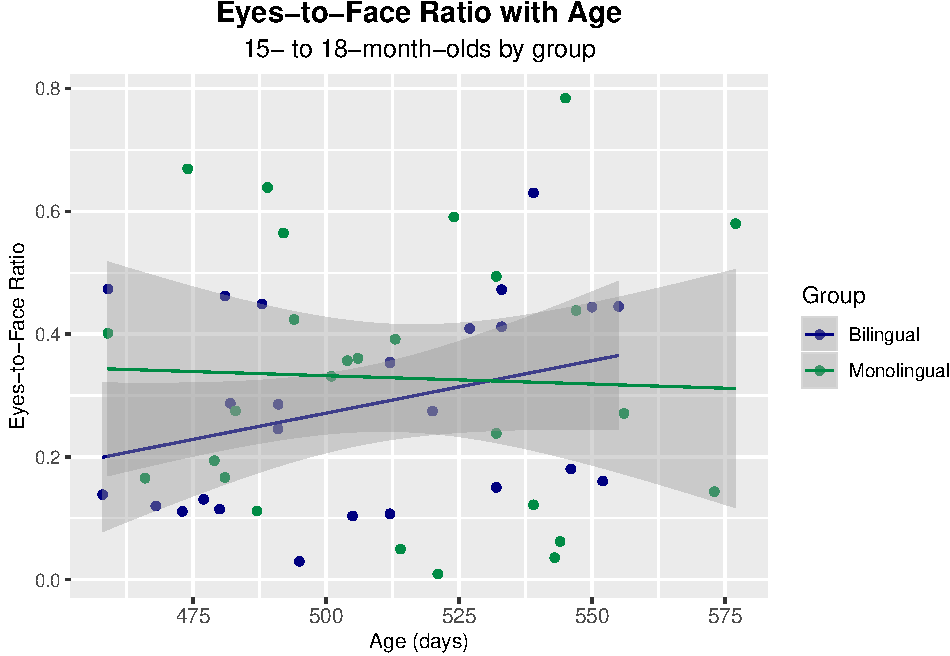
\includegraphics{Effects-of-early-language-experience-on-infants--orientation-to-faces_files/figure-latex/vm_m2fplot-1.pdf}

\hypertarget{face-orientation-index-1}{%
\subsubsection{Face Orientation Index}\label{face-orientation-index-1}}

\hypertarget{sample-1-evelynes-data-7---10-months-5}{%
\subsubsection{Sample 1 (Evelyne's Data: 7 - 10 months)}\label{sample-1-evelynes-data-7---10-months-5}}

\hypertarget{sampel-2-victorias-data-15---18-months}{%
\subsubsection{Sampel 2 (Victoria's Data: 15 - 18 months)}\label{sampel-2-victorias-data-15---18-months}}

\hypertarget{combined-sample-1-and-sample-2}{%
\subsubsection{Combined Sample 1 and Sample 2}\label{combined-sample-1-and-sample-2}}

\hypertarget{discussion}{%
\section{Discussion}\label{discussion}}

\newpage

\hypertarget{references}{%
\section{References}\label{references}}

\begingroup
\setlength{\parindent}{-0.5in}
\setlength{\leftskip}{0.5in}

\hypertarget{refs}{}
\leavevmode\hypertarget{ref-R-gridExtra}{}%
Auguie, B. (2017). \emph{GridExtra: Miscellaneous functions for "grid" graphics}. Retrieved from \url{https://CRAN.R-project.org/package=gridExtra}

\leavevmode\hypertarget{ref-R-papaja}{}%
Aust, F., \& Barth, M. (2018). \emph{papaja: Create APA manuscripts with R Markdown}. Retrieved from \url{https://github.com/crsh/papaja}

\leavevmode\hypertarget{ref-R-magrittr}{}%
Bache, S. M., \& Wickham, H. (2014). \emph{Magrittr: A forward-pipe operator for r}. Retrieved from \url{https://CRAN.R-project.org/package=magrittr}

\leavevmode\hypertarget{ref-R-Matrix}{}%
Bates, D., \& Maechler, M. (2019). \emph{Matrix: Sparse and dense matrix classes and methods}. Retrieved from \url{https://CRAN.R-project.org/package=Matrix}

\leavevmode\hypertarget{ref-R-lme4}{}%
Bates, D., Mächler, M., Bolker, B., \& Walker, S. (2015). Fitting linear mixed-effects models using lme4. \emph{Journal of Statistical Software}, \emph{67}(1), 1--48. \url{https://doi.org/10.18637/jss.v067.i01}

\leavevmode\hypertarget{ref-R-praise}{}%
Csardi, G., \& Sorhus, S. (2015). \emph{Praise: Praise users}. Retrieved from \url{https://CRAN.R-project.org/package=praise}

\leavevmode\hypertarget{ref-R-purrr}{}%
Henry, L., \& Wickham, H. (2019). \emph{Purrr: Functional programming tools}. Retrieved from \url{https://CRAN.R-project.org/package=purrr}

\leavevmode\hypertarget{ref-R-ggpubr}{}%
Kassambara, A. (2019). \emph{Ggpubr: 'Ggplot2' based publication ready plots}. Retrieved from \url{https://CRAN.R-project.org/package=ggpubr}

\leavevmode\hypertarget{ref-R-lmerTest}{}%
Kuznetsova, A., Brockhoff, P. B., \& Christensen, R. H. B. (2017). lmerTest package: Tests in linear mixed effects models. \emph{Journal of Statistical Software}, \emph{82}(13), 1--26. \url{https://doi.org/10.18637/jss.v082.i13}

\leavevmode\hypertarget{ref-R-e1071}{}%
Meyer, D., Dimitriadou, E., Hornik, K., Weingessel, A., \& Leisch, F. (2019). \emph{E1071: Misc functions of the department of statistics, probability theory group (formerly: E1071), tu wien}. Retrieved from \url{https://CRAN.R-project.org/package=e1071}

\leavevmode\hypertarget{ref-R-tibble}{}%
Müller, K., \& Wickham, H. (2019). \emph{Tibble: Simple data frames}. Retrieved from \url{https://CRAN.R-project.org/package=tibble}

\leavevmode\hypertarget{ref-R-coda}{}%
Plummer, M., Best, N., Cowles, K., \& Vines, K. (2006). CODA: Convergence diagnosis and output analysis for mcmc. \emph{R News}, \emph{6}(1), 7--11. Retrieved from \url{https://journal.r-project.org/archive/}

\leavevmode\hypertarget{ref-R-showtextdb}{}%
Qiu, Y., \& See file AUTHORS for details. (2017). \emph{Showtextdb: Font files for the 'showtext' package}. Retrieved from \url{https://CRAN.R-project.org/package=showtextdb}

\leavevmode\hypertarget{ref-R-sysfonts}{}%
Qiu, Y., \& See file AUTHORS for details. (2018). \emph{Sysfonts: Loading fonts into r}. Retrieved from \url{https://CRAN.R-project.org/package=sysfonts}

\leavevmode\hypertarget{ref-R-showtext}{}%
Qiu, Y., \& See file AUTHORS for details. (2020). \emph{Showtext: Using fonts more easily in r graphs}. Retrieved from \url{https://CRAN.R-project.org/package=showtext}

\leavevmode\hypertarget{ref-R-base}{}%
R Core Team. (2019). \emph{R: A language and environment for statistical computing}. Vienna, Austria: R Foundation for Statistical Computing. Retrieved from \url{https://www.R-project.org/}

\leavevmode\hypertarget{ref-R-broom}{}%
Robinson, D., \& Hayes, A. (2019). \emph{Broom: Convert statistical analysis objects into tidy tibbles}. Retrieved from \url{https://CRAN.R-project.org/package=broom}

\leavevmode\hypertarget{ref-R-plotly}{}%
Sievert, C. (2018). \emph{Plotly for r}. Retrieved from \url{https://plotly-r.com}

\leavevmode\hypertarget{ref-R-naniar}{}%
Tierney, N., Cook, D., McBain, M., \& Fay, C. (2019). \emph{Naniar: Data structures, summaries, and visualisations for missing data}. Retrieved from \url{https://CRAN.R-project.org/package=naniar}

\leavevmode\hypertarget{ref-R-reshape2}{}%
Wickham, H. (2007). Reshaping data with the reshape package. \emph{Journal of Statistical Software}, \emph{21}(12), 1--20. Retrieved from \url{http://www.jstatsoft.org/v21/i12/}

\leavevmode\hypertarget{ref-R-ggplot2}{}%
Wickham, H. (2016). \emph{Ggplot2: Elegant graphics for data analysis}. Springer-Verlag New York. Retrieved from \url{https://ggplot2.tidyverse.org}

\leavevmode\hypertarget{ref-R-tidyverse}{}%
Wickham, H. (2017). \emph{Tidyverse: Easily install and load the 'tidyverse'}. Retrieved from \url{https://CRAN.R-project.org/package=tidyverse}

\leavevmode\hypertarget{ref-R-forcats}{}%
Wickham, H. (2019a). \emph{Forcats: Tools for working with categorical variables (factors)}. Retrieved from \url{https://CRAN.R-project.org/package=forcats}

\leavevmode\hypertarget{ref-R-stringr}{}%
Wickham, H. (2019b). \emph{Stringr: Simple, consistent wrappers for common string operations}. Retrieved from \url{https://CRAN.R-project.org/package=stringr}

\leavevmode\hypertarget{ref-R-readxl}{}%
Wickham, H., \& Bryan, J. (2019). \emph{Readxl: Read excel files}. Retrieved from \url{https://CRAN.R-project.org/package=readxl}

\leavevmode\hypertarget{ref-R-dplyr}{}%
Wickham, H., François, R., Henry, L., \& Müller, K. (2019). \emph{Dplyr: A grammar of data manipulation}. Retrieved from \url{https://CRAN.R-project.org/package=dplyr}

\leavevmode\hypertarget{ref-R-tidyr}{}%
Wickham, H., \& Henry, L. (2019). \emph{Tidyr: Tidy messy data}. Retrieved from \url{https://CRAN.R-project.org/package=tidyr}

\leavevmode\hypertarget{ref-R-readr}{}%
Wickham, H., Hester, J., \& Francois, R. (2018). \emph{Readr: Read rectangular text data}. Retrieved from \url{https://CRAN.R-project.org/package=readr}

\leavevmode\hypertarget{ref-R-cowplot}{}%
Wilke, C. O. (2019). \emph{Cowplot: Streamlined plot theme and plot annotations for 'ggplot2'}. Retrieved from \url{https://CRAN.R-project.org/package=cowplot}

\leavevmode\hypertarget{ref-R-extrafont}{}%
Winston Chang. (2014). \emph{Extrafont: Tools for using fonts}. Retrieved from \url{https://CRAN.R-project.org/package=extrafont}

\leavevmode\hypertarget{ref-R-knitr}{}%
Xie, Y. (2015). \emph{Dynamic documents with R and knitr} (2nd ed.). Boca Raton, Florida: Chapman; Hall/CRC. Retrieved from \url{https://yihui.name/knitr/}

\leavevmode\hypertarget{ref-R-MCMCvis}{}%
Youngflesh, C. (2018). MCMCvis: Tools to visualize, manipulate, and summarize mcmc output. \emph{Journal of Open Source Software}, \emph{3}(24), 640. \url{https://doi.org/10.21105/joss.00640}

\leavevmode\hypertarget{ref-R-kableExtra}{}%
Zhu, H. (2019). \emph{KableExtra: Construct complex table with 'kable' and pipe syntax}. Retrieved from \url{https://CRAN.R-project.org/package=kableExtra}

\endgroup

\clearpage
\renewcommand{\listfigurename}{Figure captions}

\clearpage
\renewcommand{\listtablename}{Table captions}


\end{document}
